\chapter{Background of methods in order to simulate Hawkes Processes}
\label{appendix_simulate}


\section{Methods for simulating a Hawkes Process}
\label{section:definition_algo}
We describe a few algorithms for simulating Hawkes processes. We will give a particular attention to the following criteria:

\begin{itemize}
\setlength{\itemindent}{2 cm}
\item Exact (without resorting to approximation)
We refer to subsection \ref{subsection:edge} for more details about edge effect. One also defines exact as a method of drawing an unbiased associated estimator throughout the entire simulation process. \willprecise{Not sure about the meaning of exact. It would have to be checked.}
\item Efficient (no wastage, not using the rejection sampling)

\begin{definition}[Rejection Sampling]
Rejection Sampling is a basic technique used to generate observations from a distribution. One uses another distribution on a wider set $\mathcal Y$ in order to simulate values inside $\mathcal X \subset \mathcal Y$. A classic example is using a uniform distribution over a rectangle in order to create one on a circle, by rejecting all points outside the circle. 
\end{definition}

An algorithm that uses rejection sampling method is called non-efficient. 

\item Flexible (all parameters in $\Theta$ as defined previously: $ \Theta = ( \nu, \alpha, \beta ) $ )
\item Followable (source triggering the event is known)
\item Perfect (take past history into account, i.e. no "edge effect")
\item Markable (jumps can be marked; marked Hawkes process)
\item Multivariate (the algorithm supports multi-variate Hawkes process)
The criteria flexible and followable do make sense if and only if the multivariate version of the algorithm is available.
\end{itemize}


By the fact that a Hawkes process can be seen either as a non-homogeneous Poisson process or a branching process, there exists two essentials classes of simulating methods respectively: intensity based and cluster-based simulation. Intensity based methods have been studied for a long time, and many methods exists. We are going to talk about the ones that have been applied and consensual accepted in the literature. They gather into three categories: inversion, order-statistics methods and rejection sampling. We refer to \cite{gen_nonhomo_poisson} for a detailed description of the categories (a dozen algorithms are also proposed).



\subsection{Intensity based simulation}
\label{subsection:thinning}
Hawkes process generation can be viewed as the simulation of an inhomogeneous Poisson process. Indeed, the intensity is globally random, with deterministic segments in between jumps ( $\forall k \in \N, ]t_k, t_{k+1}]$ is a deterministic segment). For that reason, one can use the classic thinning algorithm (also referred to as the Lewis-Shedler thinning algorithm) whose pseudo-code can be found in \cite{lewis} and whose simplest version is well described in \cite{socialhawkes} eq. (1.18). 

Lewis' algorithm works well enough in the settings of fixed intensity functions, its main drawback is the need for a bound on the intensity that holds over an interval for all histories of the process. This, is a tremendeous flaw for applications to processes with random conditional intensities (as Hawkes processes). This difficulty has been overcomed with Ogata, whose algorithm requires only a local boundedness condition on the conditional intensity.
It is readable in \cite{Ogata} (the so called Ogata's modified thinning algorithm). 


A clear sum-up is available at the end of \cite{simullaub}. One can also find a very clear and detailed review of intensity-based algorithms in \cite{daley}, section 7.5. In particular, they mention in algorithm 7.5.II. the Lewis algorithm; algorithm 7.5.IV the Ogata's polishing and at 7.5.V. the thinning algorithm for marked point processes. 

Thinning methods fall into the category of Acceptance-Rejection methods and are not described as efficient for the reason that for $N$ events, they usually impose a complexity of $o(N^2)$. This is due to the rejection sampling method they rely on.


We write down one version of a thinning algorithm, which, as explained allows to simulate any non-homogeneous Poisson process, by knowing its deterministic intensity function:

\begin{algorithm}[H]
\label{algo:thinning_algo}
\SetAlgoLined
$t_0 = 0$,

$r_0 = 0$,

$j = 0$ and $i = 0$,

$\overline{ \lambda } = \sup_t \lambda( t ) $,

\While {$r_j < T$}
				{Sample $u \sim \text{uniform}(0,1)$, 
				
				Sample $a \sim \exp( \overline{ \lambda } )$,
				
				Set $r_{j+1} = r_j + a$,
				
				D $\sim \text{uniform}(0,1)$,
				
				\If{$ D \leq \lambda( r_{j+1} ) / \overline{\lambda} $ }
					{$t_{i+1} = r_{j+1}$,
				
					$i = i+1$,
					}
				$j = j+1$,
				}
\eIf{ $t_i \leq T$}{ return $\{t_k\}_{k = 1, \cdots, i}$. }
{ return $\{t_k\}_{k = 1, \cdots, i-1}$. }


\caption{Thinning algorithm for non-homogeneous Poisson process.}
\end{algorithm}

\begin{remarque}
Notice that instead of the condition:

\begin{align*}
D & \sim \text{uniform}(0,1) \\
\text{if } & D \leq \frac {\lambda( r_{j+1} ) } { \overline{\lambda} } 
\end{align*}


one could use equivalently:

\begin{align*}
D & \sim \text{uniform}(0, \overline{\lambda}) \\
\text{if } & D \leq \lambda( r_{j+1} ) 
\end{align*}


\end{remarque}


\begin{remarque}
Thinning algorithm relies on the idea of supremum for the intensity. For that reason, as noticed in \cite{daley}, a condition for applying such algorithm is that 

"there exists functions $M(t \mid \mathcal F_{t^-} )$ and $L(t \mid \mathcal F_{t^-} )$, such that $\forall t \in [0, \infty [$ and all list-history, the conditional intensity functions $\lambda$ of the process satisfy:

$$ 0 \leq u < L(t \mid \mathcal F_{t^-} ), \qquad  \lambda( t + u  \mid \mathcal F_{t^-} )  \leq M( t \mid \mathcal F_{t^-} )  $$

Then for any marked simple point process, the difficulty is reduced to find such functions $M,L$."


\end{remarque}

\subsection{Superposition based simulation}
Another interesting method for simulating Poisson processes is based upon the immigration-birth representation. The idea is to first simulate the immigrants as a Poisson process. Conditional on the number of immigrants, the time at which the immigrants appear is an order statistics, identically and independently uniformly distributed over the segment\footnote{One can find a proof of that in Cox-Lewis 1962, and quoted in \cite{gen_nonhomo_poisson} as theorem 2.}. The descendants then form an inhomogeneous Poisson process, which can be simulated thanks to another trick. Since we know that the branching representation of the Hawkes process has $\alpha / \beta $ births in average, we simulate the number of descendant with a Poisson law with parameter $\alpha / \beta$ and then add the new jumps by computing the inter-arrival time, immigrant-son, of an homogeneous Poisson process with parameter $\beta$.

The algorithm can be found in \cite{simullaub}. We would like however, to point-out that the algorithm is incomplete. The algorithm generates the immigrants as well as the first generation of the offspring and then stops. What should be added is a for-loop on the next generations until no new offspring is generated.




\subsection{Other Used Methods in the Literrature}
We highlight the algorithm proposed by Møller and Rasmussen \cite{rasmussen}, which is a perfect method in the sense of our definition at the beginning of the section.

An interesting evolution of thinning has been given in \cite{simuldassios}, where the authors are using superposition as well as thinning in order to reduce the complexity of the algorithm. The methods are vulgarized in \cite{socialhawkes} eq. (1.19). Basically, the authors used the Markov property of Hawkes process (granted by the exponential kernel). They also include in the algorithm the possibility of having a different starting intensity than the asymptotic underlying intensity (as previously mentioned in section \ref{section:dassios}. 

\willprecise{ exponential kernel implies markov. Mettre une référence à une section ou j'en parle mieux?}


The biggest flaw of that algorithm is that in the multivariate case, all the decays need to be identical. There is however, another algorithm that generalize \cite{simuldassios}'s one (in the sense they are also using thinning and superposition) but they did manage to get the desired flexibility. The algorithm is very well stated inside \cite{my_algo_simul}. Also, usually only cluster-based algorithm conveys information regarding the source that triggers the event times. For that reason, \cite{my_algo_simul} is an interesting algorithm on the innovative perspective.



All the previously mentioned algorithm are summed-up in the table \ref{table:methods_HP}.


\section{Pitfalls of Simulation}
\subsection{Burn-In}
\label{subsection:burn}
We want to simulate Hawkes processes over finite time windows. Unfortunately, the described methods are partially failing, as the past of the process is not known and cannot be simulated, at least not completely.

Burn-in period: for non-exact methods, a burn-in period shall be introduced to the process in order for it to reach a stationary state. Then, the effects of any transients from the initial conditions become negligible. Finding the optimal length of such period is an important question that we have not delved into.


For the sake of demonstration, we show in fig. \ref{fig:burn-in} how the burn-in impacts the process. One sees that the intensity at the beginning of the process becomes random. It is important to not include the burn-in period inside the data used for estimation. 

\begin{remarque}
Skipping the burn-in period is never recommended, though the results between the estimation given either by processes including a burn-in period or without weren't different in any significative manner.
\end{remarque}

In particular, for time-dependent parameters, the burn-in period doesn't seem to be sufficient. It was intended for reaching stationarity, though the process isn't. For that reason, in the case of time-dependent parameters, one should not change the process' parameters too quickly, or otherwise the simulation might lead to false results.

\begin{figure}
\centering
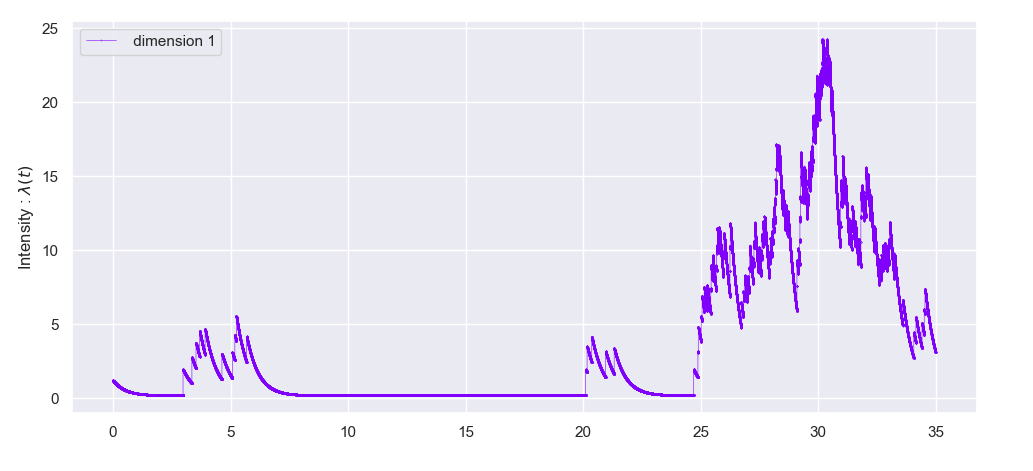
\includegraphics[width = 0.99 \textwidth]{../imag/burnin.png}
\caption{Univariate Hawkes Process with burn-in. One notices the tail of an unobserved event at the beginning of the intensity.}
\label{fig:burn-in}
\end{figure}









\begin{sidewaystable}
\begin{center}
\begin{tabular}{  | m{3.8 cm} || m{1.5 cm} |  >{\centering}m{1.7 cm}  
|| >{\centering}m{1.2 cm}  | >{\centering}m{1.52 cm}  |  >{\centering}m{1.25 cm}  |  >{\centering}m{1.6 cm}  |   >{\centering}m{2.1 cm} |  >{\centering}m{1.4 cm}  | >{\centering\arraybackslash} m{1.8 cm} | } 
\hline
Name of the Method  & Type & Author 
& Exact & Efficient 
& Perfect &  Markable & Multivariate  & Flexible & Followable  \\ 
\hline
\hline
Ozaki's Algorithm & Intensity & \cite{Ozaki} 
& $\times$ & $\checkmark$ 
& $\times$ & $\times$ & $\times$ & $-$ & $-$  \\
\hline
Thinning Algorithm & Intensity &  \cite{lewis}, \cite{simulchen}
& \checkmark & $\times $ 
& $\times$ & $\times$ & $\times$ & $-$ & $-$ \\
\hline
Ogata's Modified Thinning Algorithm & Intensity &\cite{Ogata}, \cite{simulchen}, \cite{multihawkes}
& $\checkmark$ & $\times$ 
& $\times$ & $\times$ & $\checkmark$ & \checkmark & $\times$ \\
\hline
Algorithm 7.5. Daley; & Intensity &\cite{daley}
& $\checkmark$ & $\times$ 
& $\times$ & $\checkmark$ & $\times$ & $-$ & $-$ \\
\hline
Perfect simulation & Cluster & \cite{rasmussen} 
& $\checkmark $ & $\checkmark$ 
& $\checkmark$ & $\checkmark $ & $\times$ & $-$ & $-$ \\
\hline
Exact simulation & Mixed & \cite{simuldassios} 
& $\checkmark $ & $\checkmark$ 
& $\times$ & $\checkmark $ & $\checkmark$  & $\times$ & $\times$\\
\hline
Laub's Cluster algorithm & Cluster &\cite{simullaub} 
& $\checkmark $ & $\checkmark$ 
& $\times$ & $\times$ & $\times$ & $-$ & $-$ \\
\hline
Superposed exact simulation
& Mixed & \cite{my_algo_simul} 
& $\checkmark $ & $\checkmark$ 
& $\times$ & $\checkmark $ & $\checkmark$ & $\checkmark$ & $\checkmark$ \\
\hline
\end{tabular}
\caption{Overview of a few different methods for Hawkes process simulation.}
\label{table:methods_HP}
\end{center}
\end{sidewaystable}